\chapter{Motivation}
\label{Motivation}

\emph{Mobile first} ist ein Begriff, der sich über die letzten Jahre hinweg in der Webentwicklung etabliert hat. Er bedeutet, dass zuerst für mobile Endgeräte entwickelt wird und nicht mehr die Desktop-Version im Vordergrund steht. Grund hierfür sind die zunehmenden Seitenaufrufe von Nutzern mit mobilen Endgeräten. Laut \emph{Statista} war der weltweite Anteil mobiler Endgeräte an allen Seitenaufrufen schon 2015 über 35\% \cite{statista}.

Da der Internetzugriff von mobilen Endgeräten nicht nur auf das Heimnetzwerk beschränkt bleibt, sondern auch immer mehr mit mobilen Internet genutzt wird \cite{statista:datenverkehr}, kann davon ausgegangen werden, dass die Verbindung nicht immer zuverlässig vorhanden oder langsam ist.

\begin{figure}[htb]
\centering
\caption{LTE Abdeckung der Telekom Deutschland im Raum Oberbayern}
\label{fig:netzabdeckung}
\begin{subfigure}{0.79\textwidth}
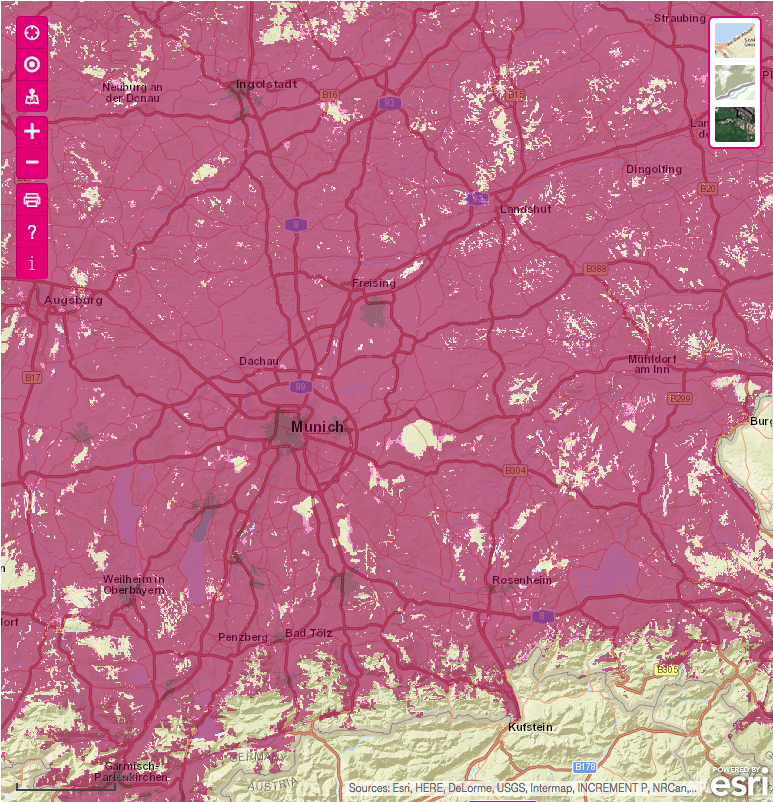
\includegraphics[width=\textwidth]{\figdir/netzabdeckung.png}
\end{subfigure}
\begin{subfigure}{0.2\textwidth}
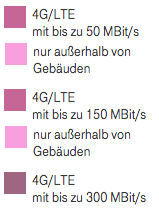
\includegraphics[width=\textwidth]{\figdir/netzabdeckung-legende.png}
\end{subfigure}
\end{figure}

In Abbildung 1.1 ist die Netzabdeckung von LTE der \emph{Telekom Deutschland} im Raum Oberbayern dargestellt. Es ist gut zu erkennen, dass selbst bei der Telekom Deutschland, die \emph{Computerbild} zufolge \cite{computerbild} die beste Netzabdeckung aufweisen kann, noch Flecken auf der Karte vorhanden sind, an denen keine LTE-Verbindung verfügbar ist.

Falls die Verbindung langsam ist bzw. abbricht, ist eine Internet-Applikation kaum zu gebrauchen, es sei denn, die Internet-Applikation ist offline-fähig. Das würde bedeuten, dass Daten offline zwischengespeichert werden können und bei erneuter Verbindung mit dem Internet synchronisiert werden können.

Genau das verspricht \emph{PouchDB}. Mit dieser Technologie können Daten im Browser persistiert werden und mit einer \emph{CouchDB} auf einem entferntem Server in Einklang gebracht werden.

Im Zuge dieser Arbeit soll PouchDB genauer beleuchtet werden und ein technischer Durchstich für eine mobile first und offline-fähige Applikation erarbeitet werden. Um diesen Durchstich zu erreichen, werden neben der CouchDB noch weitere Technologien der modernen Webentwicklung verwendet. Im nächsten Kapitel wird ein Überblick über diese Technologien gegeben.

